% LoopPilot systems position paper — Design Study + Executable Oracle Evidence
% Compile: pdflatex + bibtex + pdflatex × 2 (Windows)

\documentclass[11pt]{article}

\usepackage[utf8]{inputenc}
\usepackage[T1]{fontenc}
\usepackage{lmodern}
\usepackage{microtype}
\usepackage{amsmath,amssymb}
\usepackage{graphicx}
\usepackage{booktabs}
\usepackage{tabularx}
\usepackage{enumitem}
\usepackage{hyperref}
\usepackage{url}
\usepackage{xcolor}
\usepackage{geometry}
\geometry{margin=1in}
\usepackage{tikz}
\usetikzlibrary{arrows.meta, positioning, shapes.geometric, fit, backgrounds}
\usepackage{algorithm}
\usepackage{algorithmic}
\usepackage{array}

\hypersetup{
  colorlinks=true,
  linkcolor=blue,
  citecolor=blue,
  urlcolor=blue
}

% Shared figure palette
\definecolor{lpTask}{RGB}{41,98,150}
\definecolor{lpEvidence}{RGB}{46,125,50}
\definecolor{lpGov}{RGB}{198,90,17}
\definecolor{lpNeutral}{RGB}{245,245,248}
\definecolor{lpAccent}{RGB}{74,20,140}
\definecolor{lpLie}{RGB}{192,57,43}
\definecolor{lpAdmit}{RGB}{46,125,50}
\definecolor{lpReview}{RGB}{230,126,34}
\definecolor{lpReject}{RGB}{183,28,28}

\newcommand{\looppilot}{\textsc{LoopPilot}}
\newcommand{\cac}{\textsc{CAC}}
\newcommand{\rgr}{\textsc{RGR}}
\newcommand{\rgt}{\textsc{RGT}}
\newcommand{\sac}{\textsc{SAC}}

\title{%
  Terminal Lies in Personal AI Agents:\\
  Completion Admission Control for Long-Running Automation\\[0.4em]
  \large The \looppilot{} Position Paper
}

\author{%
  Hengji Zhang \\
  School of Computer Science, Beijing University of Posts and Telecommunications (BUPT) \\
  \texttt{bosprimigenious@bupt.edu.cn}
}

\date{\today}

\begin{document}
\maketitle

\begin{abstract}
Personal AI agents do not merely fail by producing wrong actions; they fail by producing false terminal claims.
They are deployed as long-running workflows that mutate workspaces, invoke tools, accumulate state across days, and feed later summaries, schedules, and recovery decisions.
Orchestration frameworks excel at planning and multi-step execution, yet they treat terminal success as a model-visible output rather than a runtime admission decision.
\looppilot{} reframes completion as an admission-control problem: agents may propose completion, but terminal success is admitted only when evidence has been sealed, review decisions preserved, policy boundaries checked, recovery state remains consistent, and semantic runtime acceptance oracles agree.
We call inconsistent terminal claims \textbf{terminal lies} and address them through \textbf{completion admission control (\cac{})}, the \textbf{Three-Loop Runtime Model} (Task, Evidence, Governance), and \textbf{evidence-carrying runs}, implemented in \textbf{\looppilot{}} for InternLoop, PaperLoop, and DailyNewsLoop.
This paper is a \textbf{systems position and design study with executable oracle evidence}: Codex PR~\#8 regression cases, version-pinned acceptance oracles, and a research agenda for \textbf{semantic runtime CI}.
The claim is not task-level SOTA or production safety; it is narrower and testable: terminal truthfulness can be encoded as runtime invariants over evidence bundles, review state, policy boundaries, recovery scans, and post-admission summaries.
\end{abstract}

\noindent\textbf{Keywords:} terminal lies, completion admission control, personal AI agents, evidence-carrying runs, semantic runtime CI

\section{Introduction}
\label{sec:introduction}

Personal AI agents are no longer confined to single chat sessions.
Developers delegate multi-step coding tasks overnight; researchers run literature triage across days; knowledge workers schedule information filtering before morning standups.
These workflows are \textbf{long-running}, \textbf{stateful}, and \textbf{mutating}.
The dominant research narrative emphasizes better planning, tool use, and multi-agent coordination.
That narrative is \textbf{necessary but insufficient}: when a runtime marks an unapproved patch as ``completed,'' or seals an artifact manifest before all files exist, the user loses trust not because the agent planned poorly, but because the \textbf{system lied about being done}.

Personal AI agents do not merely fail by producing wrong actions; they fail by producing false terminal claims.
\textbf{Agent completion must be admitted, not emitted.}
\looppilot{} reframes completion as an admission-control problem.

The central claim of this paper is that personal AI agents fail not only when they produce incorrect actions, but also when the runtime falsely admits those actions as completed work.
We call this failure mode a terminal lie.
Unlike ordinary task errors, terminal lies corrupt downstream trust: summaries, schedules, recovery scans, and human decisions may all treat an untrusted state as final.
\looppilot{} addresses this problem through completion admission control.
Agents may propose completion, but terminal success is admitted only when evidence has been sealed, review decisions have been preserved, policy boundaries have been checked, and semantic runtime acceptance oracles agree.
This shifts the research question from ``Can the agent finish the task?'' to ``When is the runtime allowed to say the task is finished?''

The core design principle of \looppilot{} is simple: \textbf{completion is a privilege, not a return value.}
Agents may propose outcomes; runtimes make commitments.
A terminal state is a promise to the future.
The central problem is not that agents cannot act, but that they can act without an accountable boundary for declaring completion.

Agent orchestration frameworks---LangGraph, CrewAI, AutoGen~\cite{langgraph2024,crewai2024,autogen2023}---provide hooks for human feedback at the graph level, yet typically treat terminal success, artifact integrity, and durable review state as application concerns.
In enterprise systems, governance is often distributed across platform teams, CI systems, audit logs, IAM policies, and deployment gates.
Personal automation has none of these institutional buffers; the runtime itself must govern when ``done'' may be trusted.
Evidence must precede trust.

\textbf{\looppilot{}} instantiates \cac{} as a local runtime wrapping loop implementations with explicit lifecycle states, sealed artifact bundles, SQLite-backed recovery, and a human review layer.
\looppilot{} is complementary to orchestration backends: it governs \emph{when} a run may claim success and \emph{what} evidence must exist---not \emph{how} agents plan their next step.

\subsection{Contributions}
\begin{itemize}[leftmargin=*]
  \item[\textbf{C1}] We identify terminal lies as a distinct failure mode in personal AI agent workflows.
  \item[\textbf{C2}] We propose completion admission control as a runtime principle for preventing terminal lies.
  \item[\textbf{C3}] We introduce the Three-Loop Runtime Model to separate task execution, evidence sealing, and governance admission.
  \item[\textbf{C4}] We instantiate the model in \looppilot{} and provide executable semantic runtime oracles from regression evidence.
\end{itemize}

\textbf{Positioning.} We do not claim task-level SOTA or a new general-purpose agent framework.
We claim that long-running personal automation fails through \textbf{terminal lies}---governance failures, not planning errors---that are reproducible, testable, and fixable when completion is treated as admission control.

\textbf{Mature scope.} The unit of trust in this paper is the \emph{terminal run}.
Neighboring systems admit completion claims, certify individual actions, or govern policy-constrained execution.
\looppilot{} instead asks whether a long-running personal workflow may propagate ``done'' into summaries, schedules, and recovery scans.
A correct patch can still create a terminal lie if it is summarized as completed before review admission; a safe action can still lead to untrusted terminal state if its evidence bundle is unsealed.
This scope keeps the paper out of task-SOTA competition and makes its claims executable as runtime invariants.

\textbf{Open artifact thesis.} The open-source repository is part of the scientific claim.
If reviewers cannot run the artifact, inspect the gates, or understand contribution and governance boundaries, the claim that completion is admitted by runtime evidence is weaker.
Therefore, the mature \looppilot{} paper treats open-source readiness---license, setup, contribution boundary, governance, fixtures, and reproducible commands---as an evaluation object rather than a dissemination afterthought.

\begin{figure}[t]
  \centering
  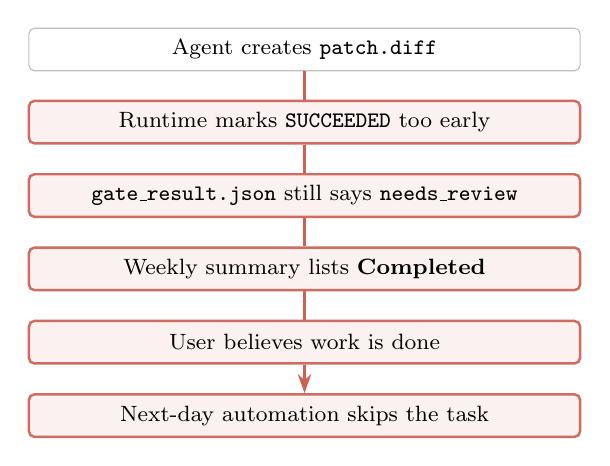
\begin{tikzpicture}[
    node distance=0.36cm,
    flowstep/.style={draw=gray!50, fill=white, rounded corners=2pt,
      minimum width=7.0cm, minimum height=0.54cm, align=center, font=\footnotesize, inner sep=4pt},
    lie/.style={flowstep, draw=lpLie!75, fill=lpLie!7, line width=0.9pt},
    arr/.style={-{Stealth[length=2.4mm,width=1.7mm]}, line width=0.95pt, draw=lpLie!80}
  ]
    \node[flowstep] (s1) {Agent creates \texttt{patch.diff}};
    \node[lie, below=of s1] (s2) {Runtime marks \texttt{SUCCEEDED} too early};
    \node[lie, below=of s2] (s3) {\texttt{gate\_result.json} still says \texttt{needs\_review}};
    \node[lie, below=of s3] (s4) {Weekly summary lists \textbf{Completed}};
    \node[lie, below=of s4] (s5) {User believes work is done};
    \node[lie, below=of s5] (s6) {Next-day automation skips the task};
    \draw[arr] (s1) -- (s2) -- (s3) -- (s4) -- (s5) -- (s6);
  \end{tikzpicture}
  \caption{How a terminal lie propagates through a personal agent workflow.
  A terminal lie is dangerous because it propagates: the wrong terminal state contaminates summaries, schedules, and future human decisions.}
  \label{fig:lie-propagation}
\end{figure}

\section{Terminal Lies: A Failure Taxonomy}
\label{sec:taxonomy}

Terminal lies are false terminal claims inconsistent with evidence, review, policy, or recovery state.
Terminal lies are not local bugs.
Once a run is falsely marked completed, the lie propagates into summaries, schedules, recovery decisions, and future task selection (Figure~\ref{fig:lie-propagation}).
Human review is not a UI event; it is durable runtime state.
We organize six recurring types discovered during 0.4 stabilization, especially Codex review on PR~\#8.
Each maps to a \looppilot{} mechanism (Table~\ref{tab:terminal-lies}).

\begin{table}[t]
  \centering
  \caption{Terminal lie taxonomy and \looppilot{} mechanisms.}
  \label{tab:terminal-lies}
  \small
  \begin{tabularx}{\linewidth}{@{}l X l@{}}
    \toprule
    \textbf{Type} & \textbf{Example} & \textbf{Mechanism} \\
    \midrule
    False Completion & Patch unapproved but summary shows completed & \rgt{} \\
    Evidence Drift & Manifest hash $\neq$ disk & \sac{} \\
    Human Decision Erasure & Deferred $\rightarrow$ pending via sync & Decision-Preserving Sync \\
    Report Misdirection & \texttt{diff-summary} as canonical report & Terminal Truthfulness \\
    Boundary Violation & Schedule install before readiness & SafetyGate \\
    Recovery Misclassification & Unsafe resume after reject & \texttt{recovery-scan} \\
    \bottomrule
  \end{tabularx}
\end{table}

\paragraph{F1 --- False completion.}
InternLoop produces \texttt{patch.diff} and passes local tests; the runtime finalizes \texttt{TERMINATED}/\texttt{SUCCEEDED} before \texttt{review approve}.
Wednesday's weekly summary lists the run under \textbf{Completed} while \texttt{gate\_result.json} reads \texttt{needs\_review}.
Trust erodes because terminal success was claimed without admission hold---a governance failure, not a planning error.
Patch existence is \textbf{evidence}; human approve is the \textbf{claim gate} for mutation.

\paragraph{F2 --- Evidence drift.}
A loop writes \texttt{artifact-manifest.json} before all artifacts exist; checksums drift when \texttt{review\_suggestion.json} is appended later.
Personal users tarball \texttt{var/artifacts/} for backup---stale hashes read as tampering.
\sac{} requires a sole finalizer that rescans disk before atomic seal.

\paragraph{F3 --- Human decision erasure.}
\texttt{review defer --until} resets to \texttt{pending} after \texttt{sync\_from\_runs}, flooding the queue.
Decision-preserving sync requires \texttt{deferred\_until} that survives sync in SQLite.

\paragraph{F4 --- Report misdirection.}
Summary logic linked \texttt{diff-summary.md} instead of canonical \texttt{report.md}.
Humans decide from Markdown; machines parse \texttt{gate\_result.json}.
Terminal truthfulness requires post-gate outcomes in traces and summaries.

\paragraph{F5 --- Boundary violation.}
Prep-stage schedule install opens unattended mutating paths before readiness checks pass.
SafetyGate enforces fail-closed prep defaults.

\paragraph{F6 --- Recovery misclassification.}
After reject, \texttt{recovery-scan} must not auto-resume unsafe runs.
Recovery state must align with terminal admission history.

\section{Completion Admission Control}
\label{sec:cac}

\textbf{Completion admission control (\cac{})} treats ``done'' as an untrusted proposal admitted by the runtime (Figure~\ref{fig:cac-pipeline}).
Completion admission control is not equivalent to adding an approval button: a button records a click; \cac{} requires sealed evidence, durable review state, policy checks, recovery consistency, and post-admission summary truthfulness before any terminal claim may propagate.
Admission requires consistency across five runtime dimensions:

\begin{enumerate}[leftmargin=*]
  \item \textbf{Completion claim} --- agent or loop proposes terminal outcome (\texttt{SUCCEEDED}, \texttt{PARTIAL}, etc.).
  \item \textbf{Evidence bundle} --- sealed artifact set with disk-recomputed checksums (\textbf{evidence-carrying run}).
  \item \textbf{Review state} --- authoritative \texttt{gate\_result.json}; human approve/reject/defer/cancel for mutating runs.
  \item \textbf{Policy state} --- SafetyGate level, ToolBroker denials, path allowlists.
  \item \textbf{Admission decision} --- runtime admits, defers, or rejects terminal success; summaries and traces reflect post-admission truth only.
\end{enumerate}

\cac{} generalizes verify-gated completion~\cite{nguyen2026verifygated}: verifiers certify step outcomes at completion time; \cac{} certifies \textbf{terminal trust across personal daily workflow}---review queues, sealed bundles, summaries, and recovery across days.

An \textbf{evidence-carrying run} turns a transient agent session into an inspectable object.
It must exit with a terminal bundle: \texttt{run\_meta.json}, \texttt{gate\_result.json}, \texttt{tool-results.json}, canonical report, \texttt{loop\_trace.jsonl}, and checksum-sealed \texttt{artifact-manifest.json} written once by the finalizer (Figure~\ref{fig:evidence-anatomy}).

\begin{figure*}[t]
  \centering
  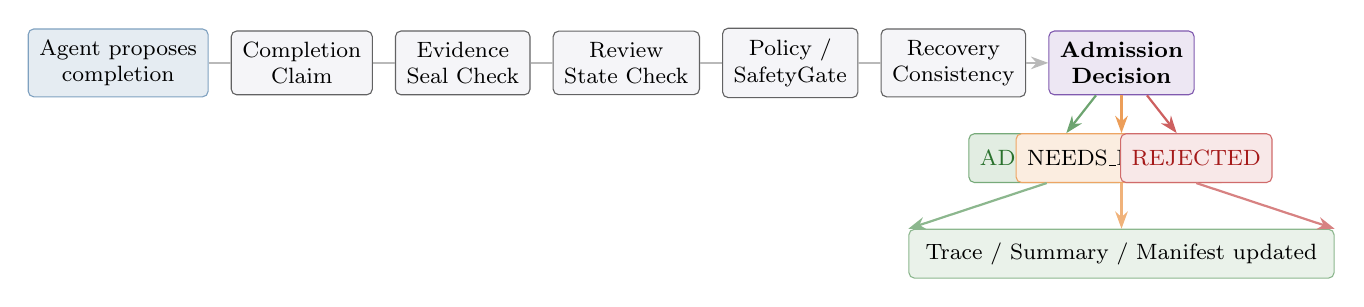
\begin{tikzpicture}[
    node distance=0.32cm and 0.28cm,
    stage/.style={draw=lpNeutral!40!black, fill=lpNeutral, rounded corners=2pt,
      minimum height=0.62cm, align=center, font=\footnotesize, inner sep=4pt},
    check/.style={stage, minimum width=1.55cm},
    start/.style={stage, fill=lpTask!12, draw=lpTask!60},
    decide/.style={stage, fill=lpAccent!10, draw=lpAccent!70, minimum width=1.7cm, font=\footnotesize\bfseries},
    outcomeA/.style={stage, fill=lpAdmit!14, draw=lpAdmit!65, minimum width=1.35cm, text=lpAdmit!90!black},
    outcomeR/.style={stage, fill=lpReview!14, draw=lpReview!70, minimum width=1.35cm},
    outcomeX/.style={stage, fill=lpReject!10, draw=lpReject!65, minimum width=1.35cm, text=lpReject!90!black},
    tail/.style={stage, fill=lpEvidence!10, draw=lpEvidence!55, minimum width=5.4cm},
    arr/.style={-{Stealth[length=2.2mm,width=1.6mm]}, thick, draw=gray!55}
  ]
    \node[start, minimum width=1.5cm] (prop) {Agent proposes\\completion};
    \node[check, right=of prop] (claim) {Completion\\Claim};
    \node[check, right=of claim] (seal) {Evidence\\Seal Check};
    \node[check, right=of seal] (rev) {Review\\State Check};
    \node[check, right=of rev] (pol) {Policy /\\SafetyGate};
    \node[check, right=of pol] (rec) {Recovery\\Consistency};
    \node[decide, right=of rec] (adm) {Admission\\Decision};
    \node[outcomeA, below=0.48cm of adm, xshift=-0.95cm] (a1) {ADMITTED};
    \node[outcomeR, below=0.48cm of adm] (a2) {NEEDS\_REVIEW};
    \node[outcomeX, below=0.48cm of adm, xshift=0.95cm] (a3) {REJECTED};
    \node[tail, below=0.58cm of a2] (tail) {Trace / Summary / Manifest updated};
    \draw[arr] (prop) -- (claim) -- (seal) -- (rev) -- (pol) -- (rec) -- (adm);
    \draw[arr, draw=lpAdmit!70] (adm) -- (a1);
    \draw[arr, draw=lpReview!75] (adm) -- (a2);
    \draw[arr, draw=lpReject!70] (adm) -- (a3);
    \draw[arr, draw=lpAdmit!55] (a1.south) -- (tail.north west);
    \draw[arr, draw=lpReview!60] (a2.south) -- (tail.north);
    \draw[arr, draw=lpReject!55] (a3.south) -- (tail.north east);
  \end{tikzpicture}
  \caption{Completion admission control pipeline.
  Terminal success flows through explicit checks; colored branches show admission outcomes.
  Only post-admission outcomes update traces, summaries, and manifests.}
  \label{fig:cac-pipeline}
\end{figure*}

\section{The Three-Loop Runtime Model}
\label{sec:three-loop}

We model personal agent runtimes as three coupled loops (Figure~\ref{fig:three-loop}):

\paragraph{Task Loop.}
Planning, tool execution, and evaluation---what orchestration frameworks optimize.
LangGraph-class planners may run inside this loop.

\paragraph{Evidence Loop.}
Artifact production, manifest sealing, checksum verification, and trace recording.
Evidence must be sealed before admission considers terminal success.

\paragraph{Governance Loop.}
Review gates, policy evaluation, SafetyGate boundaries, recovery scans, and summary truthfulness.
Governance admits or withholds terminal claims based on evidence and policy state.

Orchestration-centric designs emphasize the Task Loop; terminal lies emerge when Evidence and Governance loops are optional or decoupled.
\looppilot{} keeps all three loops coupled: no terminal admission without sealed evidence and consistent governance state.

\begin{figure}[t]
  \centering
  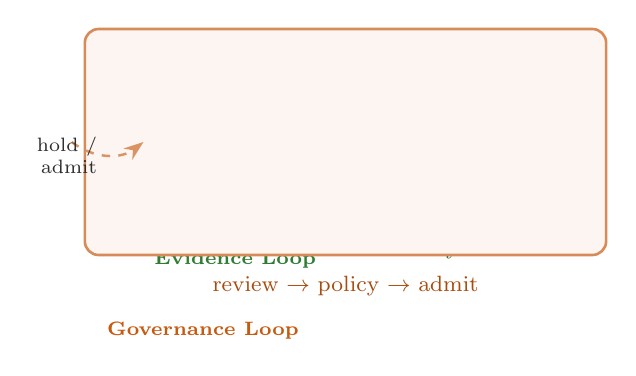
\begin{tikzpicture}[
    innerbox/.style={draw=lpTask!75, fill=lpTask!14, rounded corners=3pt,
      minimum width=4.8cm, minimum height=1.05cm, align=center, font=\small, line width=0.9pt},
    midlabel/.style={font=\scriptsize\bfseries, anchor=west},
    arr/.style={-{Stealth[length=2.5mm,width=1.8mm]}, line width=0.9pt}
  ]
    \node[innerbox] (task) {%
      \textbf{\textcolor{lpTask}{Task Loop}}\\[-1pt]
      {\footnotesize plan $\rightarrow$ act $\rightarrow$ evaluate}};
    \node[midlabel, text=lpEvidence] at ([xshift=-2.55cm,yshift=-0.95cm]task.south) {Evidence Loop};
    \node[draw=lpEvidence!70, fill=lpEvidence!8, rounded corners=4pt,
      inner sep=11pt, fit=(task), line width=0.9pt] (evfit) {};
    \node[font=\footnotesize, text=lpEvidence!85!black, align=center]
      at ([yshift=-0.42cm]evfit.south) {write $\rightarrow$ seal $\rightarrow$ verify};
    \node[midlabel, text=lpGov] at ([xshift=-3.15cm,yshift=-1.85cm]task.south) {Governance Loop};
    \node[draw=lpGov!70, fill=lpGov!6, rounded corners=5pt,
      inner sep=14pt, fit=(evfit) (evfit.south), line width=0.95pt] (govfit) {};
    \node[font=\footnotesize, text=lpGov!85!black, align=center]
      at ([yshift=-0.38cm]govfit.south) {review $\rightarrow$ policy $\rightarrow$ admit};
    \draw[arr, dashed, draw=lpGov!65] ([xshift=-0.15cm]govfit.west) to[bend right=38]
      node[left, font=\scriptsize, align=right, text=gray!35!black] {hold /\\admit} ([xshift=-0.15cm]task.west);
  \end{tikzpicture}
  \caption{Three-Loop Runtime Model (nested envelopes).
  The Task Loop may produce candidate outcomes, but only the surrounding Evidence and Governance loops can admit terminal success.}
  \label{fig:three-loop}
\end{figure}

\section{\looppilot{} Design}
\label{sec:design}

\looppilot{} implements \cac{} and the Three-Loop model through concrete components.
Table~\ref{tab:cac-mapping} maps each \cac{} dimension to \looppilot{} machinery.
Mechanisms \rgr{}, \rgt{}, \sac{}, and SafetyGate appear below as \textbf{implementation details}, not primary novelty claims.

\begin{table}[t]
  \centering
  \caption{\cac{} dimensions mapped to \looppilot{} components.}
  \label{tab:cac-mapping}
  \small
  \begin{tabular}{@{}lll@{}}
    \toprule
    \textbf{\cac{} Dimension} & \textbf{\looppilot{} Component} & \textbf{Artifact / State} \\
    \midrule
    Completion claim & RunOutcome / phase & \texttt{run\_meta.json} \\
    Evidence bundle & ArtifactStore / finalizer & \texttt{artifact-manifest.json} \\
    Review state & Review Gate & \texttt{gate\_result.json} \\
    Policy state & SafetyGate / ToolBroker & \texttt{tool-results.json} \\
    Admission decision & Orchestrator & \texttt{loop\_trace.jsonl} / summary \\
    \bottomrule
  \end{tabular}
\end{table}

\subsection{Review-Gated Runtime (\rgr{})}
The \rgr{} envelope wraps loop definitions with mandatory lifecycle phases (\texttt{CREATED} $\rightarrow$ \texttt{ACTING} $\rightarrow$ \texttt{REPORTING} $\rightarrow$ terminal states).
\texttt{RunPhase} and \texttt{RunOutcome} are independent: agent-local success does not imply admitted terminal success.

\subsection{Review-Gated Terminalization (\rgt{})}
\rgt{} blocks terminal \texttt{SUCCEEDED} for mutating runs until explicit human approve/reject/defer/cancel.
Patch runs enter \texttt{WAITING\_APPROVAL} with \texttt{PARTIAL} outcome; weekly summaries exclude them from Completed until admission.

\begin{algorithm}[t]
  \caption{Review-Gated Terminalization (admission hold)}
  \label{alg:rgt}
  \begin{algorithmic}[1]
    \REQUIRE run $r$ with optional \texttt{patch.diff}
    \IF{$r$ produces mutating artifact OR policy requires approval}
      \STATE phase $\leftarrow$ \texttt{WAITING\_APPROVAL}; outcome $\leftarrow$ \texttt{PARTIAL}
      \STATE \texttt{gate\_result.json} $\leftarrow$ \texttt{needs\_review}; exclude from Completed summary
      \STATE \textbf{wait} for human decision
      \IF{approve} \STATE admit \texttt{TERMINATED}/\texttt{SUCCEEDED}
      \ELSIF{reject or cancel} \STATE admit matching terminal outcome
      \ELSIF{defer} \STATE persist \texttt{deferred\_until}; phase $\leftarrow$ \texttt{DEFERRED}
      \ENDIF
    \ENDIF
    \STATE record post-gate event in \texttt{loop\_trace.jsonl}
  \end{algorithmic}
\end{algorithm}

\subsection{Sealed Artifact Contract (\sac{})}
The finalizer \texttt{finalize\_terminal\_artifacts()} is the sole writer of \texttt{artifact-manifest.json}.
It rescans disk, recomputes sha256 checksums, verifies required artifacts (M1--M5), and atomically seals the manifest---implementing the Evidence Loop's seal step.

\subsection{SafetyGate}
Graded safety levels (0--4) enforce fail-closed prep: unattended schedule install is blocked until readiness oracles pass.
SafetyGate addresses boundary-class terminal lies (F5).

\begin{figure*}[t]
  \centering
  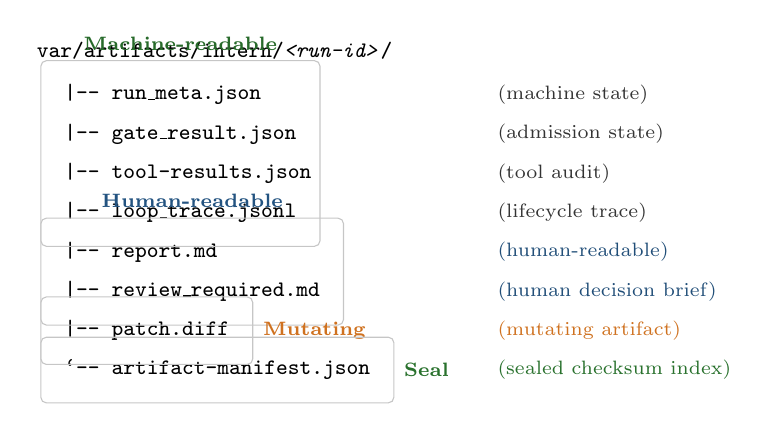
\begin{tikzpicture}[
    root/.style={font=\ttfamily\footnotesize, anchor=west},
    file/.style={root, text=black},
    tag/.style={font=\scriptsize, text=gray!40!black, anchor=west},
    bracket/.style={draw=gray!45, rounded corners=2pt}
  ]
    \node[file] (r0) at (0,0) {var/artifacts/intern/\textit{<run-id>}/};
    \node[file] (r1) at (0.35,-0.55) {|-- \texttt{run\_meta.json}};
    \node[tag] at (5.85,-0.55) {(machine state)};
    \node[file] (r2) at (0.35,-1.05) {|-- \texttt{gate\_result.json}};
    \node[tag] at (5.85,-1.05) {(admission state)};
    \node[file] (r3) at (0.35,-1.55) {|-- \texttt{tool-results.json}};
    \node[tag] at (5.85,-1.55) {(tool audit)};
    \node[file] (r4) at (0.35,-2.05) {|-- \texttt{loop\_trace.jsonl}};
    \node[tag] at (5.85,-2.05) {(lifecycle trace)};
    \node[file] (r5) at (0.35,-2.55) {|-- \texttt{report.md}};
    \node[tag, text=lpTask!80!black] at (5.85,-2.55) {(human-readable)};
    \node[file] (r6) at (0.35,-3.05) {|-- \texttt{review\_required.md}};
    \node[tag, text=lpTask!80!black] at (5.85,-3.05) {(human decision brief)};
    \node[file] (r7) at (0.35,-3.55) {|-- \texttt{patch.diff}};
    \node[tag, text=lpReview!90!black] at (5.85,-3.55) {(mutating artifact)};
    \node[file] (r8) at (0.35,-4.05) {`-- \texttt{artifact-manifest.json}};
    \node[tag, text=lpEvidence!90!black] at (5.85,-4.05) {(sealed checksum index)};
    \node[bracket, fit=(r1)(r4), inner sep=5pt, label={[font=\scriptsize\bfseries, text=lpEvidence!85!black]above:Machine-readable}] {};
    \node[bracket, fit=(r5)(r6), inner sep=5pt, label={[font=\scriptsize\bfseries, text=lpTask!85!black]above:Human-readable}] {};
    \node[bracket, fit=(r7), inner sep=5pt, label={[font=\scriptsize\bfseries, text=lpReview!90!black]right:Mutating}] {};
    \node[bracket, fit=(r8), inner sep=5pt, label={[font=\scriptsize\bfseries, text=lpEvidence!90!black]right:Seal}] {};
  \end{tikzpicture}
  \caption{Evidence-carrying run anatomy.
  A terminal bundle couples machine-readable admission state, human-readable decision briefs, mutating artifacts, and a sealed checksum index.}
  \label{fig:evidence-anatomy}
\end{figure*}

\subsection{A Walkthrough: From Patch Generation to Admitted Completion}
\label{sec:walkthrough}

We trace an InternLoop morning repair through all three loops.
The walkthrough shows how \cac{} prevents a terminal lie when the Task Loop believes the repair is done but governance has not yet admitted completion.

\paragraph{Task Loop (steps 1--5).}
(1)~The user starts an InternLoop morning run.
(2)~The agent reads a failed \texttt{pytest} log and plans a fix.
(3)~ToolBroker allows test execution under policy.
(4)~The agent generates \texttt{patch.diff}.
(5)~The Task Loop evaluates local tests and \emph{thinks} the repair is done---but this is only a completion \textbf{proposal}.

\paragraph{Evidence Loop (step 6).}
(6)~The Evidence Loop writes \texttt{tool-results.json}, canonical \texttt{report.md}, \texttt{loop\_trace.jsonl}, and prepares the manifest for sealing.
Evidence must precede trust; no admission decision consults agent prose alone.

\paragraph{Governance Loop (steps 7--9).}
(7)~The Governance Loop detects a mutating artifact (\texttt{patch.diff}).
(8)~\rgt{} holds terminal success: phase $\rightarrow$ \texttt{WAITING\_APPROVAL}, outcome $\rightarrow$ \texttt{PARTIAL}.
(9)~The run enters \texttt{needs\_review}; \texttt{gate\_result.json} is authoritative.
Human review is not a UI event; it is durable runtime state persisted alongside the bundle.

\paragraph{Admission and summary (steps 10--11).}
(10)~The weekly summary does \textbf{not} list the run under Completed---terminal truthfulness excludes unadmitted runs.
(11)~After the user issues \texttt{review approve}, the runtime admits \texttt{TERMINATED}/\texttt{SUCCEEDED}, seals the manifest, and only then updates summary membership.
Agents may propose outcomes; runtimes make commitments.

\paragraph{Loop case studies.}
\textbf{InternLoop} --- development patches trigger \rgt{}; patch existence is evidence, human approve is the claim gate.
\textbf{PaperLoop} --- claim-evidence governance blocks writes without sources.
\textbf{DailyNewsLoop} --- signal-to-action boundary keeps triage non-mutating; candidates flow to inbox for deliberate action.

\section{Executable Oracle Evidence and Research Agenda}
\label{sec:evidence}

This section reports \textbf{version-pinned} acceptance evidence and \textbf{design-study} regression cases---not full benchmark results.
Evidence is divided into two classes: executed acceptance oracles that are safe to cite for the named snapshot, and proposed benchmark protocols that remain future work.

\subsection{Regression Evidence from PR \#8}
Codex automated review on PR~\#8 surfaced seven governance engineering issues mapping to terminal lie types F1--F6: false completion, stale manifest, report misrouting, suggestion ordering, trace dishonesty, deferred sync regression, and approve/resume ambiguity.
Each became a named regression test---\textbf{failure-driven design evidence}, not a benchmark score.
Historical pre-PR~\#8 behavior exhibited F1: patch runs reached \texttt{TERMINATED}/\texttt{SUCCEEDED} while \texttt{gate\_result.json} still read \texttt{needs\_review}.

\subsection{Measured Acceptance Oracles}
Table~\ref{tab:acceptance-measured} records commands executed on 2026-06-22.
Newer repository badges must not be cited in this paper until the same gates are rerun and the commit hash is pinned.

\begin{table}[t]
  \centering
  \caption{Measured acceptance oracle results (2026-06-22).}
  \label{tab:acceptance-measured}
  \small
  \begin{tabular}{@{}lll@{}}
    \toprule
    \textbf{Check} & \textbf{Command} & \textbf{Result} \\
    \midrule
    Lint & \texttt{ruff check .} & pass \\
    Unit + integration & \texttt{pytest -q} & 227 passed \\
    0.4 aggregate & \texttt{verify\_0\_4\_acceptance.py} & 11/11 READY \\
    0.4-c review layer & \texttt{verify\_0\_4c\_acceptance.py} & 36/36 READY \\
    \bottomrule
  \end{tabular}
\end{table}

These oracles encode subsets of governance invariants as executable checks.
They demonstrate that terminal-lie fixes are testable without claiming task-level SOTA.

\subsection{Semantic Runtime CI (Research Agenda)}
\textbf{Semantic runtime CI} extends traditional CI: verify semantic consistency of runtime claims---phase/outcome pairs, gate files, manifest checksums, summary membership, defer persistence---not merely that unit tests pass.
Traditional CI asks whether code tests pass.
Semantic runtime CI asks whether the runtime is allowed to say that the workflow passed.
Table~\ref{tab:semantic-ci} (Appendix) sketches oracle mappings; measured acceptance oracles in Table~\ref{tab:acceptance-measured} encode subsets of these invariants today.
We outline benchmark protocols (gate correctness, manifest integrity, recovery preservation, safety boundaries, cross-loop coverage, overhead profiling, daily-use trials) as future semantic runtime CI suites; full protocol execution remains future work.
Metric abbreviations are deferred to Appendix~\ref{app:metrics}; RQ-style protocol sketches appear in Appendix~\ref{app:rq-protocols}.

\subsection{Mature Evaluation Path}
\label{sec:mature-eval}

The full-paper path is to convert acceptance oracles into fault-injection suites and executable ablations.
GateBench injects patch-review faults and measures false completion.
ArtifactTruthBench injects stale manifests and missing required artifacts.
RecoveryFaultBench exercises defer, reject, and resume histories.
SafetyBoundaryBench attempts forbidden unattended scheduling and mutation.
DailyUseBench measures whether summaries remain actionable across repeated runs.
This path turns the position claim into a systems result without requiring task-level SOTA claims.
Table~\ref{tab:pr8-fault-map} shows the first consolidated map from PR~\#8 findings to injectable faults and expected blocks.

\begin{table*}[t]
  \centering
  \caption{PR~\#8 fault-injection map for semantic runtime CI.}
  \label{tab:pr8-fault-map}
  \small
  \begin{tabularx}{\linewidth}{@{}p{0.08\linewidth} X X X@{}}
    \toprule
    \textbf{ID} & \textbf{Injected fault} & \textbf{Oracle / guard} & \textbf{Expected block} \\
    \midrule
    FI-1 & Patch run finalizes \texttt{SUCCEEDED} while gate is \texttt{needs\_review} & 0.4-c review tests; aggregate gate & Hold at \texttt{WAITING\_APPROVAL}/\texttt{PARTIAL} \\
    FI-2 & Manifest written before all artifacts exist & Terminal artifact tests & Finalizer recomputes disk state before seal \\
    FI-3 & Manifest includes itself & Manifest self-exclusion assertion & Self-entry rejected \\
    FI-4 & \texttt{diff-summary.md} promoted as canonical report & Report path priority test & Canonical loop report selected \\
    FI-5 & Review suggestion written after finalization & Checksum inclusion test & Suggestion written before finalizer \\
    FI-6 & Terminal trace appended before review downgrade & Trace truthfulness assertion & Trace records post-gate state \\
    FI-7 & Deferred review item reset to pending during sync & Review sync preservation test & \texttt{deferred\_until} survives sync \\
    FI-8 & Approved patch treated as resume request & Approve/resume behavior test & Approve directly admits terminal success \\
    FI-9 & Prep-stage schedule install allowed & SafetyGate prep tests & Install/unattended path denied \\
    \bottomrule
  \end{tabularx}
\end{table*}

\subsection{Open Artifact Readiness}
\label{sec:open-artifact}

Artifact review standards distinguish whether artifacts are evaluated, available, and independently validated.
\looppilot{} should target the first two before submission: a reviewer should be able to start from a clean checkout, run the WSL setup, execute acceptance oracles, inspect generated artifacts, and understand who may change safety policy.
Table~\ref{tab:open-artifact-gate} turns open-source practice into a paper gate.

\begin{table}[t]
  \centering
  \caption{Open-source artifact gate for an A-level \looppilot{} submission.}
  \label{tab:open-artifact-gate}
  \small
  \begin{tabularx}{\linewidth}{@{}>{\bfseries}p{0.23\linewidth} X@{}}
    \toprule
    Layer & Required evidence \\
    \midrule
    License & Explicit root license and artifact license statement. \\
    Setup & WSL path, Python environment, API bridge, mobile client, and full validation commands. \\
    Contribution & Contribution guide that explains tests, SafetyGate boundaries, and review expectations. \\
    Governance & Maintainer authority, release gate, artifact-claim gate, and safety-policy change process. \\
    Reproducibility & Pinned commit, command log, expected outputs, fixtures, and generated artifact bundle. \\
    \bottomrule
  \end{tabularx}
\end{table}

\section{Discussion}
\label{sec:discussion}

Personal AI agents do not merely fail by producing wrong actions; they fail by producing false terminal claims.
\looppilot{} reframes completion as an admission-control problem: \textbf{agent completion must be admitted, not emitted.}
\textbf{Completion is a privilege, not a return value.}
A terminal state is a promise to the future; personal habit formation depends on summaries and schedules reflecting post-admission truth only.

\paragraph{Workshop positioning.}
This paper is a \textbf{systems position and design study with executable oracle evidence}, not an empirical benchmark paper.
We name terminal lies and \cac{} to sharpen workshop discourse beyond ``add human approval'' (Figure~\ref{fig:comparison}, Appendix).

\paragraph{Scope.}
\looppilot{} targets personal single-user deployment without enterprise ops teams.
Governance artifacts serve local audit needs rather than fleet monitoring~\cite{mlflow2024,opentelemetry2024}.

\paragraph{Complementarity.}
LangGraph interrupt/resume resembles \texttt{WAITING\_APPROVAL}, but lacks system-wide summary exclusion, deferred persistence, and sole-writer manifest sealing~\cite{langgraph2024}.

\paragraph{Operational lessons.}
Codex-driven redesign shows terminal lies are reproducible when acceptance scripts encode invariants as oracles.

\section{Threats to Validity}
\label{sec:threats}

\paragraph{Internal validity.}
The strongest evidence in this paper is executable but fixture-heavy: unit tests, acceptance scripts, and PR~\#8 regression oracles exercise semantic runtime invariants under controlled local conditions.
These checks are appropriate for terminal truthfulness because the claim concerns runtime state consistency, not open-ended task quality.
However, they can miss failures caused by long tool latencies, operating-system differences, or real adapter behavior.

\paragraph{External validity.}
\looppilot{} is a single-user personal runtime.
The design deliberately avoids enterprise assumptions such as centralized audit teams, IAM policy services, or multi-party approval chains.
As a result, the paper should not be read as evidence that \cac{} is sufficient for organization-scale governance.
The transferable claim is narrower: long-running personal agents need a runtime admission layer before terminal success propagates to summaries, schedules, and recovery.

\paragraph{Construct validity.}
The measured oracles evaluate false completion, manifest integrity, review-state preservation, safety-boundary blocking, and summary truthfulness.
They do not measure task-level correctness, user satisfaction, or production reliability.
The fault-injection bench currently binds PR~\#8 findings to non-mutating oracles; explicit source/workspace mutation remains future work and is therefore not reported as benchmark coverage.

\paragraph{Artifact validity.}
The open-source artifact now includes governance documents, WSL setup, static API/mobile checks, and a clean-checkout artifact review bundle generator.
This improves inspectability, but reproducibility still depends on a reviewer-provided Python 3.11+ environment and network access for dependency installation after checkout.
Version-pinned paper claims must be refreshed only after rerunning the recorded commands at a pinned commit.

\section{Related Work}
\label{sec:related}

\paragraph{Agent orchestration.}
LangGraph, CrewAI, and AutoGen optimize the Task Loop~\cite{langgraph2024,crewai2024,autogen2023}.
They rarely mandate evidence-carrying runs, checksum-sealed manifests, or durable review queues.
Checkpointing pauses graphs; it does not enforce terminal truthfulness on weekly summaries.

\paragraph{Verify-gated completion.}
Recent work treats task completion as verifier admission: a run claims ``done'' only after executable verification passes~\cite{nguyen2026verifygated}.
Nguyen and Tran study verify-gated completion as admission control in a governed multi-agent runtime, separating execution from a read-only verifier that admits or rejects completion claims with packetized evidence and fail-closed defaults.
Such systems gate \emph{step-level} or \emph{claim-level} completion at verification time.
\looppilot{} validates \textbf{terminal trust across personal daily workflow}: review state, artifact bundles, summary membership, and recovery scans across days---not only whether a single verification event passed at completion time.

\paragraph{Proof-carrying agent actions.}
Proof-Carrying Agent Actions (PCAA) organize runtime governance around action certificates with checkpoints for pre-action admissibility, action open, assumption capture, approval, and outcome closure~\cite{wang2026pcaa}.
PCAA binds portable envelopes, runtime receipts, and replay-ready proof to individual actions across heterogeneous agent runtimes.
The trust object is \textbf{action-level}: each certificate attests what was authorized and what evidence accompanied a specific action.
\looppilot{} provides a \textbf{run-level evidence-carrying terminal bundle}: sealed manifests, gate files, and post-admission summaries that certify whether the \emph{run} may be trusted as finished---complementary to action certificates, not a substitute.

\paragraph{Policy-constrained execution and governance by construction.}
Policy-constrained execution frameworks externalize governance into a runtime layer that mediates agent-proposed actions through capability admission, policy checking, and rollback handling~\cite{qin2026policy}.
SARC and related governance-by-architecture approaches compile regulatory and enterprise obligations into runtime constraints at declared enforcement sites in the agent loop~\cite{besanson2026sarc}.
These lines of work protect \textbf{action safety} and \textbf{enterprise policy checkpoints}---blocking unsafe tool use, enforcing compliance predicates, and routing escalations to human operators.
\looppilot{} targets \textbf{terminal truthfulness} for single-user long-running automation without an ops team: defer persistence, manifest sealing, and summary truthfulness so personal habit formation is not corrupted by false ``done'' states.
SafeAgent-style benchmarks~\cite{safeagent2024} similarly emphasize unsafe \emph{actions}; terminal lies can persist even when every action was individually safe.

\paragraph{Software-engineering agents.}
SWE-agent and SWE-bench optimize patch correctness~\cite{yang2024sweagent,jimenez2024swebench}.
High pass@k does not prevent terminal lies if summaries falsely mark unapproved patches complete.

\paragraph{Artifact evaluation.}
Artifact evaluation traditions emphasize reproducible packages~\cite{icse2019repeatability}.
\looppilot{} seals artifacts \emph{per run at runtime} for daily personal workflows.

\section{Conclusion}
\label{sec:conclusion}

Personal AI agents do not merely fail by producing wrong actions; they fail by producing false terminal claims.
\looppilot{} reframes completion as an admission-control problem.
\textbf{Agent completion must be admitted, not emitted.}
\textbf{Completion admission control} addresses terminal lies through the \textbf{Three-Loop Runtime Model} and \textbf{evidence-carrying runs}, instantiated in \looppilot{} with executable semantic runtime oracles from regression evidence (11/11 aggregate; 227 pytest passed in the version-pinned 2026-06-22 snapshot).
Future work executes semantic runtime CI benchmark suites and completes controlled-real E2E evaluation.

\section*{Acknowledgments}
The author thanks Codex automated review on PR~\#8 for surfacing terminal-lie blockers during 0.4 stabilization.

\bibliographystyle{plain}
\bibliography{references}

\appendix
\section{Extended Metric Definitions}
\label{app:metrics}

Table~\ref{tab:app-metrics} lists metric abbreviations for planned semantic runtime CI protocols.

\begin{table}[h]
  \centering
  \caption{Appendix metrics for benchmark protocols (not measured in main text).}
  \label{tab:app-metrics}
  \small
  \begin{tabular}{@{}lll@{}}
    \toprule
    \textbf{Symbol} & \textbf{Name} & \textbf{Protocol} \\
    \midrule
    FCR & False Completion Rate & InternLoop-GateBench \\
    MIR & Manifest Integrity Rate & ArtifactTruthBench \\
    HDPR & Human Decision Preservation Rate & RecoveryFaultBench \\
    UMBR & Unsafe Mutation Block Rate & SafetyBoundaryBench \\
    DAR & Daily Actionability Rate & Daily trial \\
    \bottomrule
  \end{tabular}
\end{table}

\section{RQ Protocol Summary}
\label{app:rq-protocols}

Seven research questions (RQ1--RQ7) sketch semantic runtime CI protocols: review-gate correctness, manifest integrity, recovery preservation, safety boundaries, cross-loop coverage, governance overhead, and daily-use trials.
Execution remains future work; measured acceptance oracles in Section~\ref{sec:evidence} encode subsets of RQ1--RQ5 invariants.

\section{Supplementary Figures and Tables}
\label{app:figures}

\begin{figure}[ht]
  \centering
  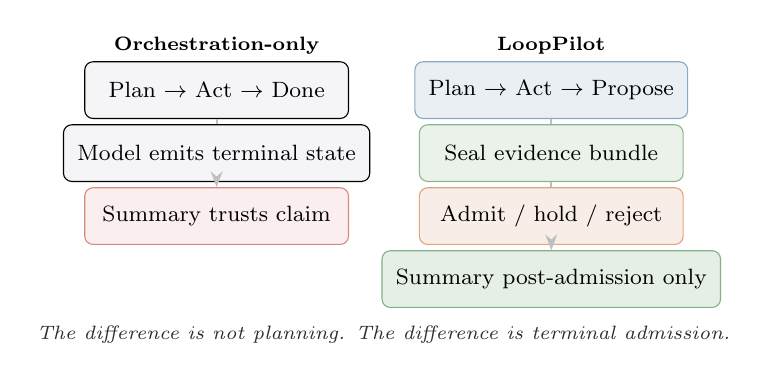
\begin{tikzpicture}[
    col/.style={draw, rounded corners=3pt, minimum width=3.35cm, minimum height=0.72cm,
      align=center, font=\footnotesize, inner sep=5pt},
    lane/.style={font=\scriptsize\bfseries, anchor=north},
    arr/.style={-{Stealth[length=2mm]}, thick, draw=gray!50}
  ]
    \node[lane] at (0, 1.55) {Orchestration-only};
    \node[lane] at (4.25, 1.55) {\looppilot{}};
    \node[col, fill=lpNeutral] (o1) at (0, 0.75) {Plan $\rightarrow$ Act $\rightarrow$ Done};
    \node[col, fill=lpNeutral] (o2) at (0, -0.05) {Model emits terminal state};
    \node[col, fill=lpLie!8, draw=lpLie!60] (o3) at (0, -0.85) {Summary trusts claim};
    \node[col, fill=lpTask!10, draw=lpTask!55] (l1) at (4.25, 0.75) {Plan $\rightarrow$ Act $\rightarrow$ Propose};
    \node[col, fill=lpEvidence!10, draw=lpEvidence!55] (l2) at (4.25, -0.05) {Seal evidence bundle};
    \node[col, fill=lpGov!10, draw=lpGov!55] (l3) at (4.25, -0.85) {Admit / hold / reject};
    \node[col, fill=lpAdmit!12, draw=lpAdmit!60] (l4) at (4.25, -1.65) {Summary post-admission only};
    \draw[arr] (o1) -- (o2) -- (o3);
    \draw[arr] (l1) -- (l2) -- (l3) -- (l4);
    \node[font=\scriptsize\itshape, text=gray!35!black, align=center]
      at (2.12,-2.35) {The difference is not planning. The difference is terminal admission.};
  \end{tikzpicture}
  \caption{\textbf{Figure A1.} Orchestration-only vs.\ \looppilot{} terminal handling.
  Planning is necessary in both columns; only \cac{} separates proposal from admitted completion.}
  \label{fig:comparison}
\end{figure}

\begin{figure}[ht]
  \centering
  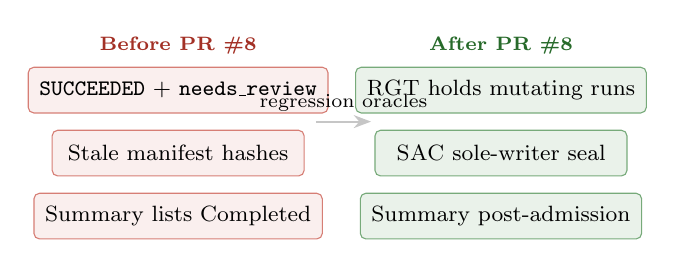
\begin{tikzpicture}[
    col/.style={rounded corners=2pt, minimum width=3.2cm, minimum height=0.58cm,
      align=center, font=\footnotesize, inner sep=4pt},
    lane/.style={font=\scriptsize\bfseries, anchor=north}
  ]
    \node[lane, text=lpLie!85!black] at (0, 1.35) {Before PR \#8};
    \node[lane, text=lpAdmit!85!black] at (4.1, 1.35) {After PR \#8};
    \node[col, draw=lpLie!65, fill=lpLie!8] (b1) at (0, 0.55) {\texttt{SUCCEEDED} + \texttt{needs\_review}};
    \node[col, draw=lpLie!65, fill=lpLie!8] (b2) at (0, -0.25) {Stale manifest hashes};
    \node[col, draw=lpLie!65, fill=lpLie!8] (b3) at (0, -1.05) {Summary lists Completed};
    \node[col, draw=lpAdmit!65, fill=lpAdmit!10] (a1) at (4.1, 0.55) {\rgt{} holds mutating runs};
    \node[col, draw=lpAdmit!65, fill=lpAdmit!10] (a2) at (4.1, -0.25) {\sac{} sole-writer seal};
    \node[col, draw=lpAdmit!65, fill=lpAdmit!10] (a3) at (4.1, -1.05) {Summary post-admission};
    \draw[-{Stealth[length=2.2mm]}, thick, draw=gray!45] (1.75,0.15) -- (2.45,0.15)
      node[midway, above, font=\scriptsize] {regression oracles};
  \end{tikzpicture}
  \caption{\textbf{Figure A2.} PR~\#8 failure-driven redesign.
  Codex review surfaced terminal lies that became named acceptance oracles.}
  \label{fig:pr8-redesign}
\end{figure}

\begin{table}[ht]
  \centering
  \caption{\textbf{Table A3.} Semantic runtime CI oracle matrix (sketch).}
  \label{tab:semantic-ci}
  \small
  \begin{tabular}{@{}lll@{}}
    \toprule
    \textbf{Runtime Claim} & \textbf{Evidence Checked} & \textbf{Oracle} \\
    \midrule
    Completed & \texttt{gate\_result} $\neq$ \texttt{needs\_review} & \texttt{verify\_0\_4} \\
    Report link & canonical report exists & report\_path test \\
    Manifest seal & sha256 matches disk & manifest validation \\
    Defer preserved & \texttt{deferred\_until} unchanged & review sync test \\
    Safe scheduling & install blocked & SafetyGate test \\
    \bottomrule
  \end{tabular}
\end{table}

\end{document}
